\chapter{Design Milestone \\
  \small{\textit{-- Evan Ciok, Sophia DiCuffa, Carson McManus}}
  \index{Chapter!designMilestone}
  \index{Design Milestone}
  \label{Chapter::designMilestone}}

\section{Problem Statement}

This project aims to model and overhaul the architecture of OpenTogetherTube, a platform for watching videos with
friends. The current OTT system runs on node.js, which runs JavaScript code in a single thread. An event loop exists
with the function of handling incoming requests, but this can get backed up as the number of clients to handle
increases. This leads to response times that can be far higher than desired for a responsive platform like OTT.
A vertical or horizontal approach can be taken in an effort to alleviate the overbearing load. Vertical scaling
of the system, like optimizing network usage, would be effective, but there is an imposed ceiling on its impact.
Horizontal scaling on the other hand has no such ceiling. By introducing more instances of the backend via
node.js on new processing units the load can be distributed and handled much more efficiently. This architectural
remodel would allow OTT to gain the capacity for large scale expansion moving forward.

Tagline: Horizontal Scaling for OpenTogetherTube

\section{Project Description}

OpenTogetherTube is a user-friendly real time video platform that allows users to watch videos together with their
friends. The website boasts a stellar suite of features, including synchronized playback, a voting system, and
playlist copying. Upon launching the site the user is met with a simple interface and clear options to either
browse or create a room. These rooms can house a dynamic number of users via public joining or dedicated share links,
and they can join at any time. Each room has a video player which synchronously runs the video and audio for all
users and accepts links from a multitude of platforms such as YouTube, Vimeo, and Dailymotion. Videos can be put
into a queue one at a time or through entire playlist links, and a room voting system for the next video can be used
alternatively to the default queue.

In order to eliminate friction from the user experience, OTT allows full usage from guest users, while providing extra
benefits to regular users who opt to create a login with the platform. Once a user has logged in, permanent rooms can
be created that receive dedicated URLs so a group can hop in and out whenever they please. The system's interactive UI
is built on a Vue frontend, which is a JavaScript framework that extends standard HTML and CSS. This project will focus
on the refactoring of the backend, where all server-side programming is handled by Node.js. In its current state, OTT's
architecture is inefficient and not fitting for long term scalability. The largest constraint on the system right now is
the increased load per additional user on the Node event loop. By approaching this issue with a horizontal scaling tactic
of being able to spin up and take down nodes as needed, the overall load could be handled in a more efficient way. In
order to achieve this, smart load balancers can be used to make room assignments under the context of knowing each node's
current load. Doing so would distribute traffic evenly and prevent overload failure or bottlenecking, increasing response
time and availability for users.


\section{Use Cases}

\subsection{Project Maintainer}

The primary use case is that the project maintainer(s) need to be able to quickly and easily add new nodes to the system.

OTT's production deployment is on Heroku, which is a PaaS (Platform as a Service) that allows you to deploy your application to the
cloud in containers called dynos. Dynos are isolated, virtualized Linux containers that are designed to execute code based on a
user-specified command.

The process of scaling the service up and down needs to be reasonably automated, and it needs to be compatible with Heroku's dynos.

\subsection{End User}

The end user's use case is to be able to join a room and watch a video with their friends. Ultimately, the end user should not be
able to tell that the system is horizontally scaled. The UI shouldn't change at all.

\section{Design Sketches}

There are four sequence flows to display our design in action. First, there is joining a room (Figure \ref{Figure::room}). Next, there is joining an unloaded room (Figure \ref{Figure::unloaded}). Then, there is generating and joining a temporary room (Figure \ref{Figure::temp}). Last, we have creating and joining a new named temporary room, our edge case (Figure \ref{Figure::edge}).

\begin{figure}
  \centering
  \scalebox{0.7}{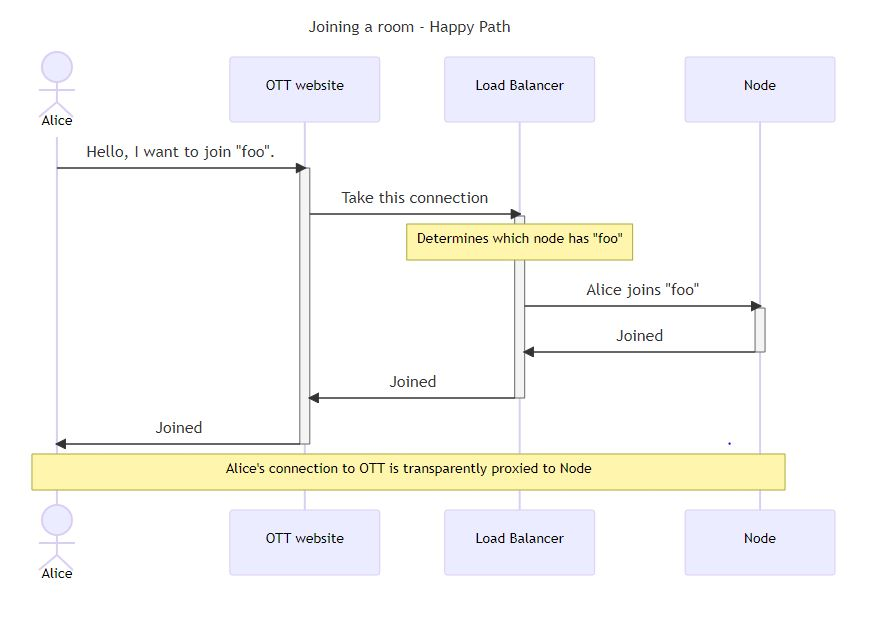
\includegraphics{Figures/designMilestone/room.jpg}}
  \caption{\label{Figure::room} Joining a room.}
\end{figure}

\begin{figure}
  \centering
  \scalebox{0.7}{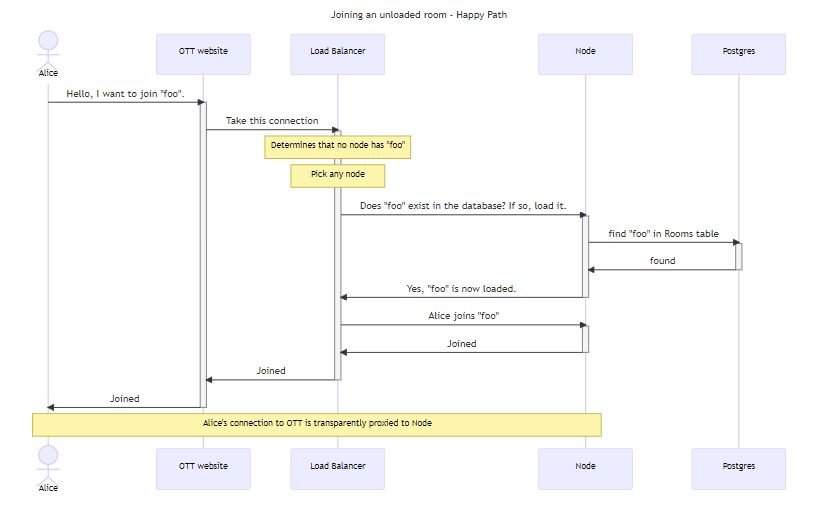
\includegraphics{Figures/designMilestone/unloaded.jpg}}
  \caption{\label{Figure::unloaded} Joining an unloaded room.}
\end{figure}

\begin{figure}
  \centering
  \scalebox{0.7}{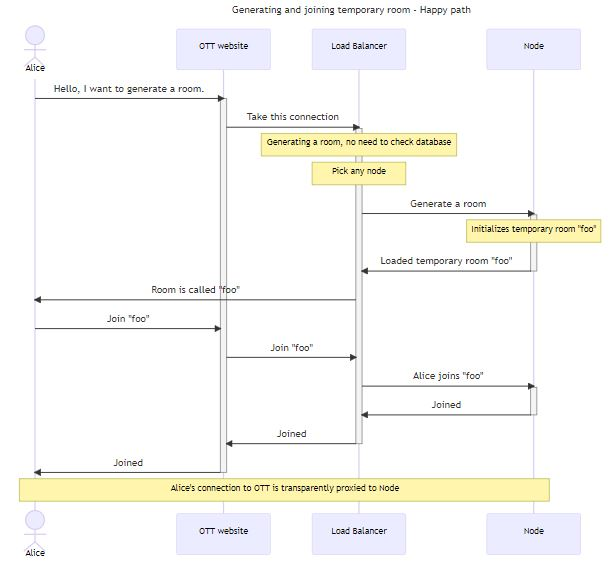
\includegraphics{Figures/designMilestone/temp.jpg}}
  \caption{\label{Figure::temp} Generating and joining a temporary room.}
\end{figure}

\begin{figure}
  \centering
  \scalebox{0.7}{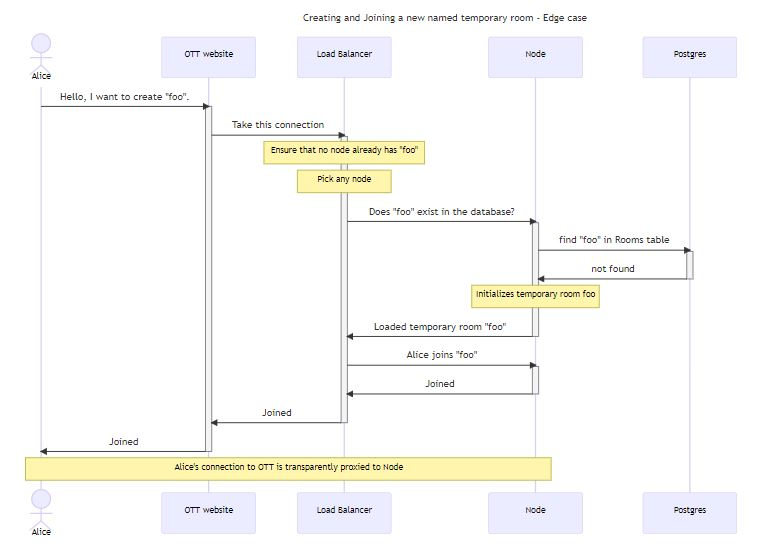
\includegraphics{Figures/designMilestone/edge.jpg}}
  \caption{\label{Figure::edge} Generating and joining a new named temporary room.}
\end{figure}


\newpage

\section{Architecture Design}

OTT's current architecture (Figure \ref{Figure::old-architecture}) is a single node.js monolith, backed by Redis
for caching, pubsub, and login sessions, and PostgreSQL for persistent
storage, and video metadata caching.

\begin{figure}[htb]
  \centering
  \scalebox{0.5}{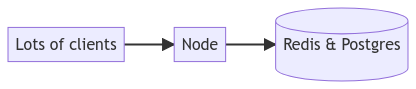
\includegraphics{Figures/designMilestone/architecture-old.png}}
  \caption{\label{Figure::old-architecture} Current Configuration}
\end{figure}

In the new proposed configuration (Figure \ref{Figure::new-architecture}), all
load balancers would maintain their own hash table of rooms. When a client
wants to join a room, the load balancer would check its hash table for the
room. If the room is loaded, the connection is forwarded to the node that
has the room loaded. If the room is not loaded, the balancer will pick a node,
and ask if there is a matching unloaded permanent room. If the room is not found,
the connection is closed.

\begin{figure}[htb]
  \centering
  \scalebox{0.5}{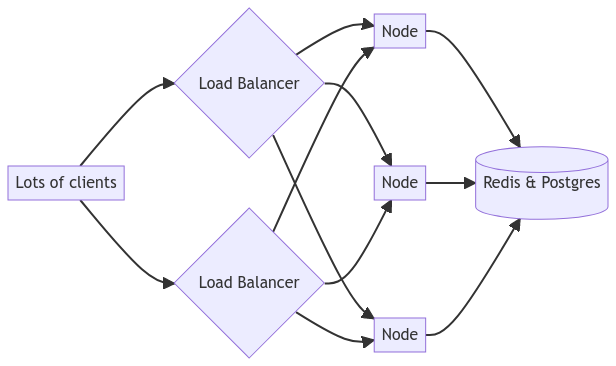
\includegraphics{Figures/designMilestone/architecture-new.png}}
  \caption{\label{Figure::new-architecture} Proposed Configuration}
\end{figure}

To reduce resource usage, the load balancers would only maintain a single
connection to each node. This means that the load balancers need to wrap the
messages sent by clients so that the node can identify the client that sent
the message, and which room the message was for. The load balancer would need
to also need to maintain a mapping of which clients have joined which rooms.
The nodes would also need to maintain a mapping of which clients have joined
from which load balancers so that if a load balancer fails, the node can clean
up the clients that were connected to it.

\begin{figure}[htb]
  \centering
  \scalebox{0.6}{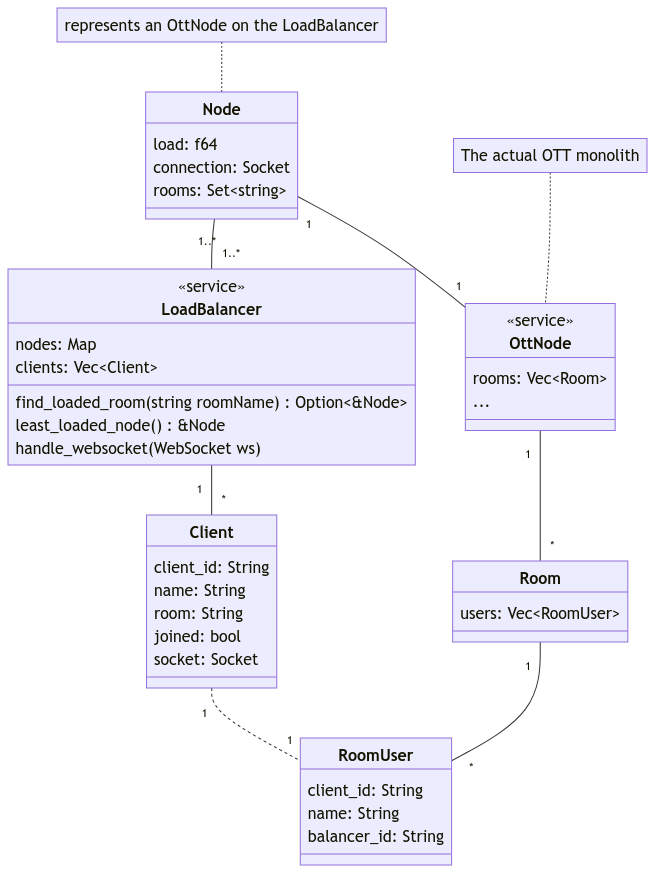
\includegraphics{Figures/designMilestone/uml-load-balancer.png}}
  \caption{\label{Figure::uml-load-balancer} Proposed Code Structure for Load Balancer}
\end{figure}
